\subsection{Recurrent Neural Network}

\begin{frame}[fragile]
\frametitle{Recurrent Neural Network}

\begin{itemize}
\item Bekommen sowohl von Eingangssignale sowohl durch Trainingsdatensatz als auch durch Rückkopplungen. 
\end{itemize}

\begin{columns}
\hspace{10mm}

\begin{column}{.6\textwidth}

\begin{figure}
	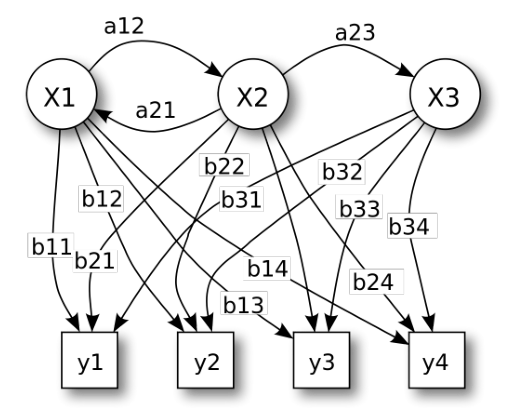
\includegraphics[width=\linewidth]{./zusatz/recurrentNN/img/rnn_aufbau_alpha}
\end{figure}

\end{column}
\begin{column}{.4\textwidth}

\vspace{-24mm}

\begin{itemize}
\item Mustererkennung
\item Muster ergänzen
\item Sprachanalyse
\end{itemize}
\end{column}

\end{columns}

\note[item]{Bisher nur feedforward NN
\begin{itemize}
    \item Eingangssignale ohne Bezug auf vorherige Durchläufe
\end{itemize}}

\note[item]{Hierbei Reihenfolge von Bedeutung
\begin{itemize}
    \item RNNs bekommen sowohl Eingagssignale durch den Trainingsdatensatz als auch durch Rückkopplungen während der Ausführung
\end{itemize}}

\note[item]{Viele Anwendungsbereiche
\begin{itemize}
    \item besonders gut um Muster zu erkennen bzw. zu Ergänzen
    \item aber auch in der Sprachanalyse sehr wichtig
\end{itemize}}

\end{frame}
